%%%%%%%%%%%%%%%%%%%%%%%%%%%%%%%%%%%%%%%%%%%%%%%%%%%%%%%
%\subsubsection{Unpolarised PDFs}
%\label{sec:unpPDFs}

%We present the global PDF fitiing framework, and discuss how PDFs are extracted
%from hard-scattering cross-sections, paying special attention
%to the assessment of the PDF uncertainties.
%
%We also briefly discuss the state-of-the-art for unpolarised
%global PDF fits.
%%
%Throughout this section,
%we have made an effort to use a notation fully consistent
%with the previous lattice-QCD discussion.

%\paragraph{General framework}
%
%Unpolarised PDFs appear in the factorisation formulae for both
%deep-inelastic scattering (DIS) and for proton-proton collisions.
%
%The factorised expression of the unpolarised DIS structure functions 
%was given in Eq.~\eqref{eq:Fi}.
%
%For the hadroproduction of a generic final-state $X$ in $pp$ collisions, we hav%e
%a corresponding factorised expression
%\begin{equation}
%  \label{eq:LHCxsec}
%\sigma_{pp\to X}(s,\mu_F,\mu_R)=\sum_{a,b}\int {\rm d}x_1 {\rm d}x_2\, f_a(x_1,%\mu_F^2)f_b(x_2,\mu_F^2)\,\hat{\sigma}_{ab\to X}(x_1,x_2,s;\mu_{F},\mu_R)\;,
%\end{equation}
%where the hard cross section $\hat{\sigma}_{ab\to X}$ can
%be calculated perturbatively as an expansion in the QCD and EW running coupling%s.
%%
%The specific values of the momentum fractions
%$x_i$ are related to the kinematics of the final state.
%%
%In particular, at leading order it can be shown that
%\be
%x_{1,2}=\frac{M_X}{\sqrt{s}}e^{\pm y_X} \, ,
%\ee
%where $M_X$, $y_X$ are the invariant mass and rapidity of the produced system r%espectively.
%%
%The factorisation and renormalisation scales, $\mu_F$ and $\mu_R$, are taken to% be of order of the hard scale,
%$\mu_F,\mu_R \sim Q$, of the process.
%
%The DGLAP evolution equations of the PDFs, Eq.~(\ref{eq:dglapunp}), 
%ensure that, when performing a global fit, the PDFs can be parameterised at 
%one arbitrary (perturbative) input scale $Q_0\sim 1$ GeV, and
%then be connected to any other higher scale $\mu$ that might be relevant
%for comparisons with experimental data.
%%
%This input PDF parameterisation takes the generic form
%\begin{equation}
%\label{eq:pdffunc}
%f(x,Q_0,\{a_i\})\sim x^{a_1}(1-x)^{a_2}\:C(x,\{a_{i>2}\})\, ,
%\end{equation}
%where the parameters $\{a_i\}$ determine the PDF shape
%and are different for each PDF flavour combination that
%is extracted from the data.
%%
%The $(1-x)^{a_2}$ term, with $a_{2}>0$, ensures that the PDFs
%vanish in the elastic $x\to 1$ limit, as we would expect on basic physical grou%nds. 
%%
%Such a behaviour is also expected from the quark
%counting rules~\cite{Brodsky:1973kr,Ball:2016spl}.
%%
%The $x^{a_1}$ term, which dominates in the low $x$
%region, is expected from general Regge theory considerations,
%although in modern fits the value of the power itself is left free.
%
%The interpolating function $C(x)$ in
%Eq.~\eqref{eq:pdffunc}
%affects the behaviour of the PDFs away from the $x\to 0$ and 1
%extrapolation regions.
%%
%This is assumed to be a smoothly varying function of $x$, for which a variety o%f choices have been made in PDF fits, as we discuss below.
%%
%The heavy quark PDFs $c(x,\mu)$ and $b(x,\mu)$ are usually not
%parameterised using the form in  Eq.~\eqref{eq:pdffunc}, but rather
%generated by perturbative emission of gluons and light quarks,
%though it is also possible to fit the charm PDF on an equal footing
%to the light quarks~\cite{Ball:2016neh}.
%
%While the general $x$ dependence of the PDFs is determined by
%non-perturbative QCD dynamics, there are still a number
%of theoretical constraints that any PDF set should satisfy and thus that
%should be imposed during the global fit.
%%
%First of all, since
%the proton has the quantum numbers of two up quarks and one down quark,
%we have the following quark number sum rules given in terms of zeroth
%moments: 
%
%\begin{eqnarray}
%\int_{0}^{1}dx\ \left[u(x,\mu)-\bar{u}(x,\mu)\right] & =\left\langle 1\right\rang%le _{u^{-}}= & 2 \, ,\nonumber \\
%\int_{0}^{1}dx\ \left[d(x,\mu)-\bar{d}(x,\mu)\right] & =\left\langle 1\right\rang%le _{d^{-}}= & 1 \, ,
%\label{eq:valencesumrules}\\
%\int_{0}^{1}dx\ \left[s(x,\mu)-\bar{s}(x,\mu)\right] & =\left\langle 1\right\rang%le _{s^{-}}= & 0 \, ,\nonumber
%\end{eqnarray}
%with similar constraints for the heavy quarks: $\left\langle 1\right\rangle _{c^{%-}}=\left\langle 1\right\rangle _{b^{-}}=\left\langle 1\right\rangle _{t^{-}}=0$.
%%
%Note that these constraints hold for any scale $\mu$, and indeed it can be shown
%that if they hold at the input parametrisation scale $Q_0$, they
%are subsequently respected by DGLAP evolution.
%%
%Therefore, for these distributions we must have $a_1>-1$ for the exponents in
%Eq.~(\ref{eq:pdffunc}), else the valence sum rules would be ill-defined.

%The second sum rule that we can impose on the PDFs arises
%from the basic conservation of energy-momentum derived from
%the QCD Lagrangian.
%%
%This so-called momentum sum rule arises
%because the proton's total momentum should be equal to the sum of the momentum
%carried by all its constituents, namely
%\begin{equation}\label{eq:mom}
%1 = \left\langle x\right\rangle _{g}+\left\langle x\right\rangle _{u^{+}}+\left\la%ngle x\right\rangle _{d^{+}}+\left\langle x\right\rangle _{s^{+}}+\left\langle x\ri%ght\rangle _{c^{+}}+\left\langle x\right\rangle _{b^{+}}+\left\langle x\right\rangl%e _{t^{+}}+\ldots\,,
%\end{equation}
%%
%where the ellipsis represents any other partonic components (such
%as a photon). The zeroth moments, $\left\langle x\right\rangle _{f_i}$, are defin%ed in analogy to Eq.~\eqref{eq:umoment1} and \eqref{eq:uplusmoment1}. Thus for n%on--valence distributions, we must have $a_1>-2$ to avoid a divergent contributi%on to
%Eq.~\eqref{eq:mom}; typically we have $-2<a_1<-1$ for such distributions, and th%erefore for small $x$ the number of soft partons
%grows very quickly, although the momentum fraction carried by them is well-defin%ed
%and finite.
%%
%As in the case of the valence sum rules, the momentum
%sum rule is preserved by the DGLAP evolution equations.

%As a representative illustration of the results of a global
%PDF analysis, in Fig.~\ref{fig:nnlopdfs} we show
%the results of the PDF4LHC15 NLO set~\cite{Butterworth:2015oua}
%both at a low scale
%    $\mu^2=Q^2=4~{\rm GeV}^2$  and at
%    $\mu^2=Q^2=10^2~{\rm GeV}^2$.
%    %
%    Specifically, we show the  $u_v=u-\bar{u}$ and $d_v=d-\bar{d}$ valence combi%nations, the $\bar{u}$,
%    $\bar{d}$, $s$ and $c$ sea quark PDFs, and the gluon (divided by a factor 10%).
%    %
%    Recall that the evolution between $Q^2=10$ to $Q^2=10^4~{\rm GeV}^2$ is comp%letely
%    determined by the solution of
%     the DGLAP evolution equations.
%    %
%    Note how the shape of the $u_v~(u^{-})$ and $d_v~(d^{-})$ valence quark combi%nations
%    reflects the constraints from the valence sum rules Eq.~(\ref{eq:valencesumr%ules}).
%    %
%    At small $x$, there is a rapid growth of the gluon and the sea quark PDFs, i%mplying
%    that the higher the collision center-of-mass energy $\sqrt{s}$, the more
%    important gluon- and sea-quark-initiated processes become.
%    %
%    The bands in Fig.~\ref{fig:nnlopdfs} represent the 68\% confidence level (CL%)
%    PDF uncertainties, determined as discussed below.
%
%%%%%%%%%%%%%%%%%%%%%%%%%%%%%%%%%%%%%%%%%%%%%%%%%%%%%%%%%%%%%%%%%%%%%%
%\begin{figure}[t]
%\begin{center}
%  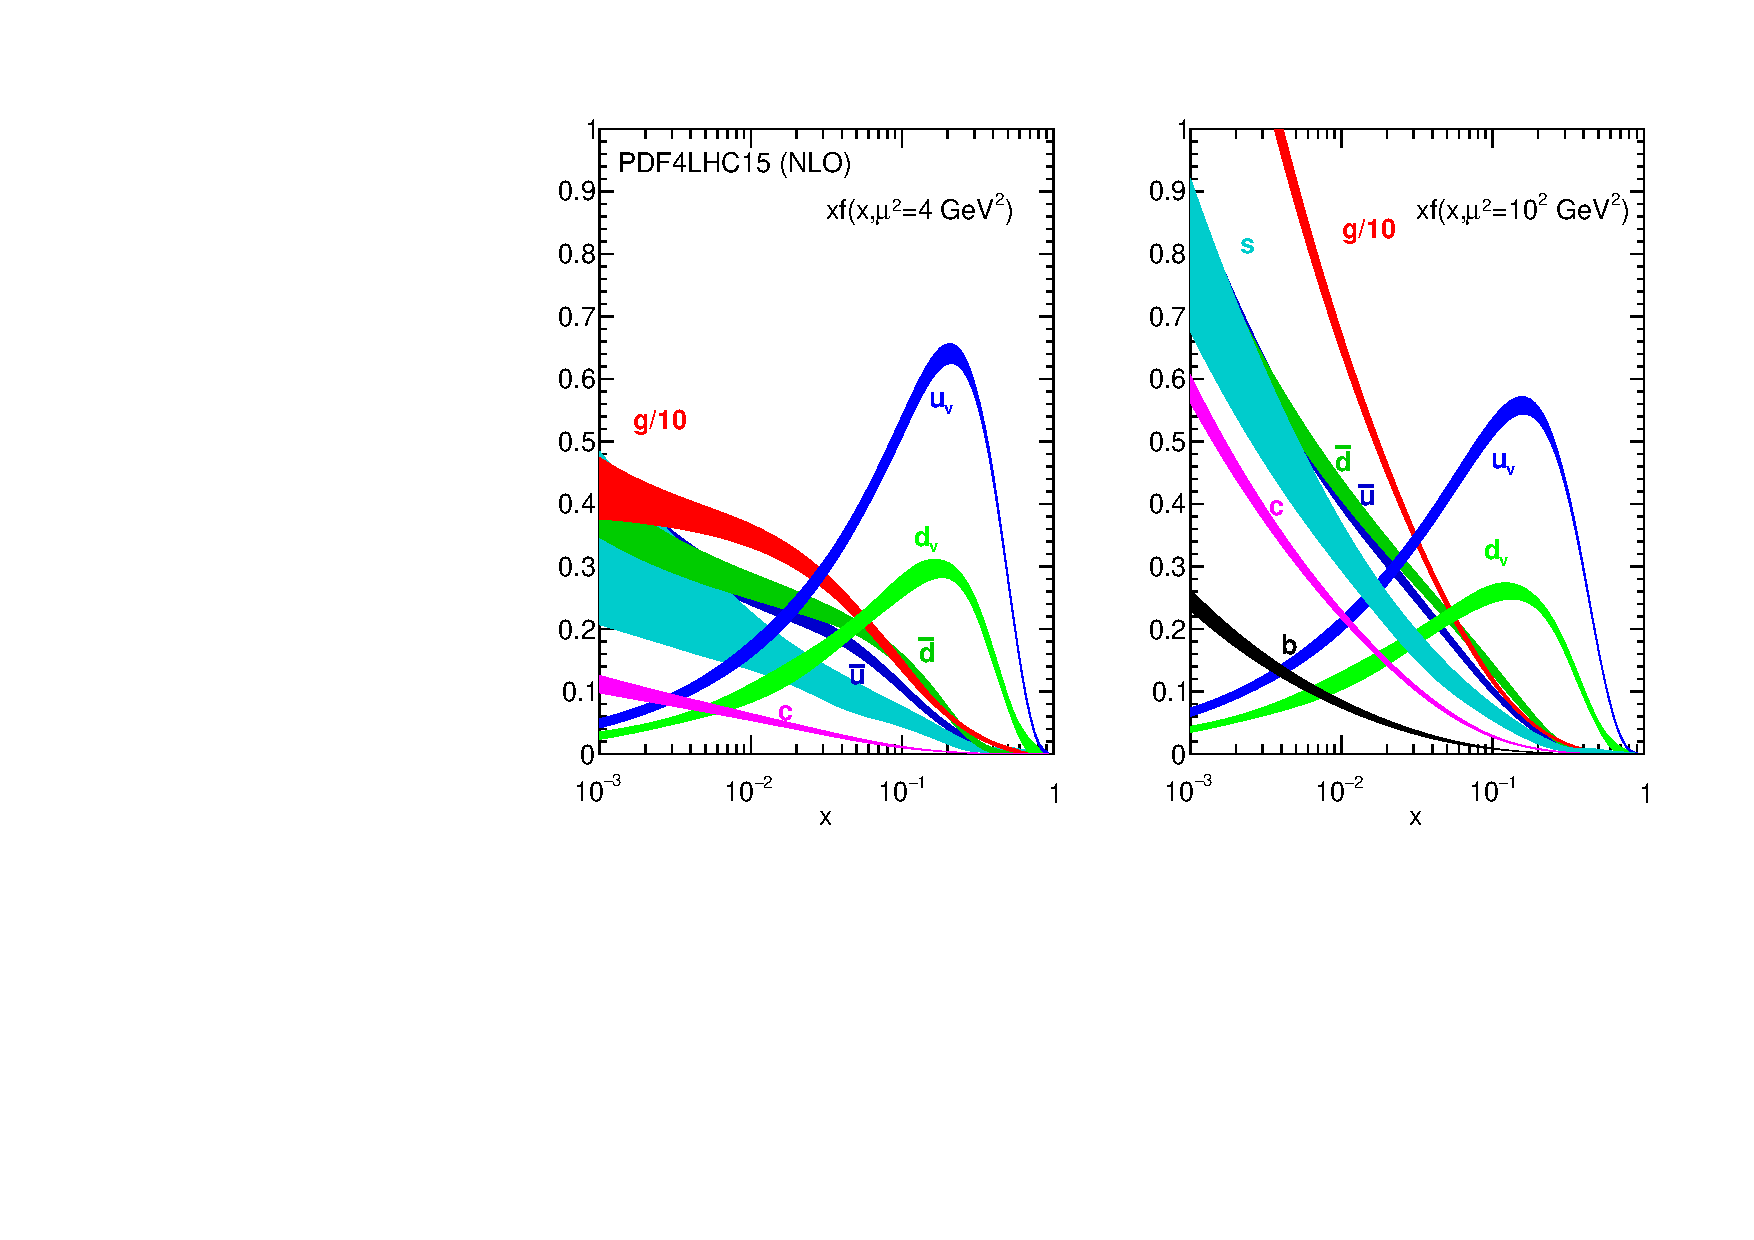
\includegraphics[scale=0.8]{plots/PDF4LHC15.pdf}\\
%  \caption{\small The PDF4LHC15 NLO PDFs at a low scale
%    $\mu^2=Q^2=4~{\rm GeV}^2$ (left plot) and at 
%    $\mu^2=Q^2=10^2~{\rm GeV}^2$ (right plot) as a function of $x$.
%    %
%    We show the $u_v$ and $d_v$ valence combinations, the $\bar{u}$,
%    $\bar{d}$, $s$ and $c$ sea quark PDFs, and the gluon (note that
%    the latter is divided by a factor 10).
%    \label{fig:nnlopdfs}
%  }
%\end{center}
%\end{figure}
%%%%%%%%%%%%%%%%%%%%%%%%%%%%%%%%%%%%%%%%%%%%%%%%%%%%%%%%%%%%%%%%%%%%%%%

%\paragraph*{Fitting PDFs from hard-scattering data.}
%
%The global PDF analysis framework is based on a combination of three basic comp%onents: experimental
%data, perturbative calculations, and fitting methodology, which we now describe
%in turn.

%\begin{enumerate}
%\item A broad set of input hard-scattering cross-sections from DIS and proton-p%roton collisions, providing information on the PDFs
%  over a wide range of $x$ and for different flavour combinations.
%  %
%  While traditional PDF fits were based mostly on DIS structure function and Dr%ell-Yan
%  and inclusive jet
%  cross-sections, in recent years many other processes have proved important fo%r constraining PDFs, from top-quark pair production~\cite{Czakon:2016olj}
%  to the $p_T$ of $Z$ bosons~\cite{Boughezal:2017nla}
%  and $D$ meson production in the forward region~\cite{Gauld:2016kpd}. %, among%  several others.
%
%  In Fig.~\ref{fig:kinplot-report} we show the representative kinematic coverag%e in the
%    $(x,Q^2)$ of the DIS and proton-proton hard-scattering measurements that ar%e
%    used as input in a global unpolarised PDF fit, in this case NNPDF3.1~\cite{%Ball:2017nwa}.
%    %
%    In order to facilitate visualisation, different
%    datasets have been clustered together into families of
%    related processes.
%    %
%      For hadronic cross-sections, leading order kinematics are assumed to map
%    each experimental bin to a pair of points in the $(x,Q^2)$ plane.
%    %
%    We observe that the current dataset extends down to $x\simeq 5\cdot 10^{-5}%$
%    at low $x$, and up to few TeV at high $Q^2$.
%    %
%    The fact that similar regions in the $(x,Q^2)$ plane are covered by
%    different processes is essential to achieve quark
%    flavour separation and to constrain the gluon PDF.
%
%%%%%%%%%%%%%%%%%%%%%%%%%%%%%%%%%%%%%%%%%%%%%%%%%%%%%%%%%%%%%%%%%%%%
%\begin{figure}[t]
%\begin{center}
%  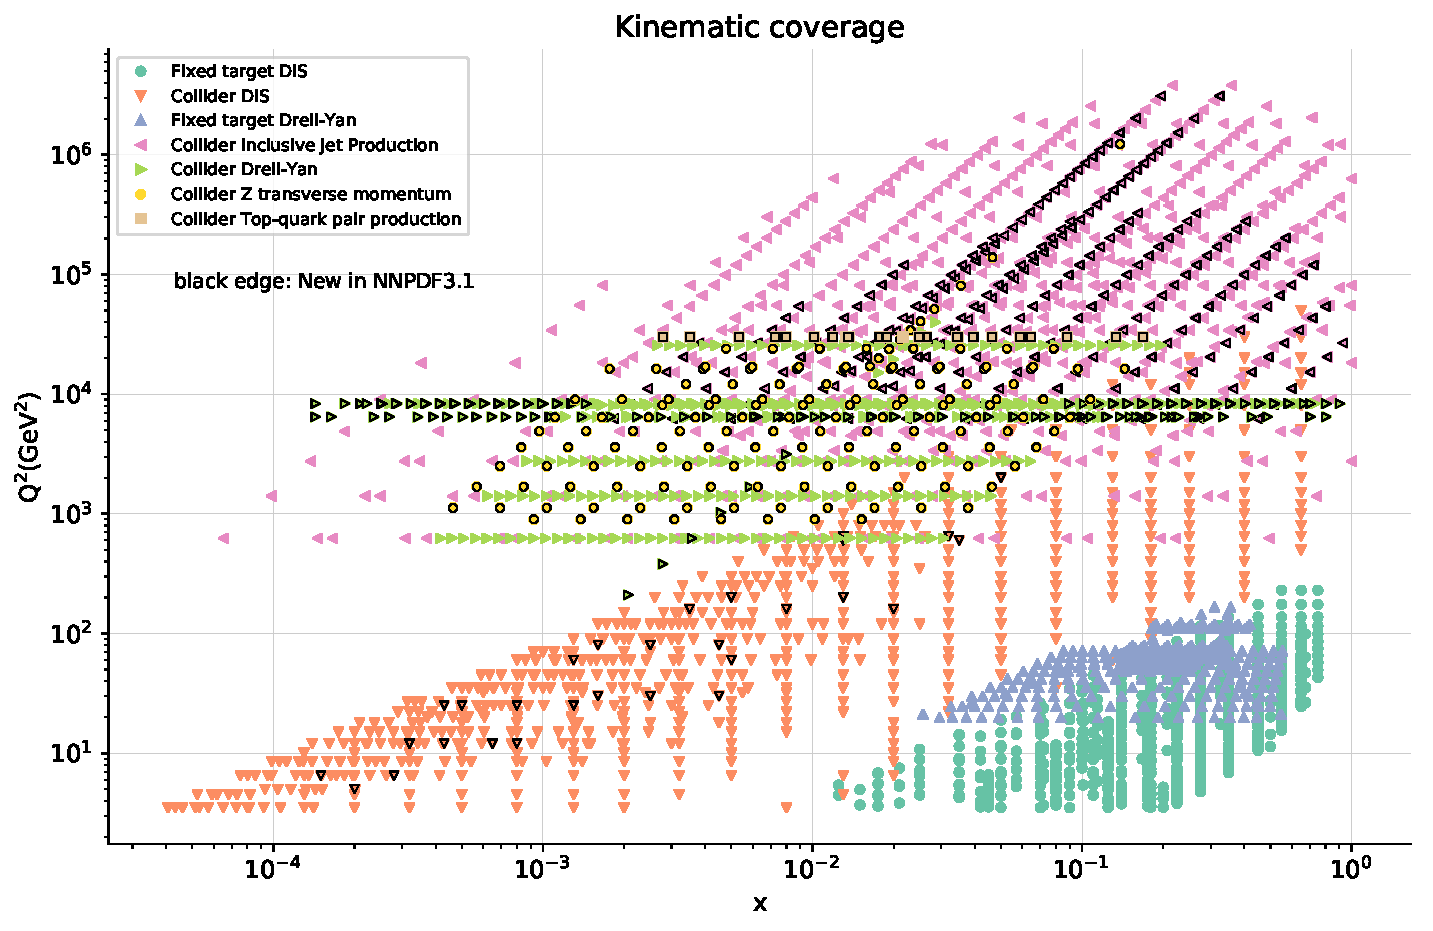
\includegraphics[scale=0.60]{plots/kinplot-report.pdf}
%  \caption{\small Representative kinematical coverage in the
%    $(x,Q^2)$ of the DIS and proton-proton hard-scattering measurements that ar%
%    used as input in a global unpolarised PDF fit, in this case NNPDF3.1~\cite{%Ball:2017nwa}.
%    %
%    In order to facilitate visualisation, different
%    datasets have been clustered together into families of
%    related processes.
%    %
%    For hadronic cross-sections, leading order kinematics are assumed to map
%    each experimental bin to a pair of points in the $(x,Q^2)$ plane.
%    \label{fig:kinplot-report} 
%  }
%\end{center}
%\end{figure}
%%%%%%%%%%%%%%%%%%%%%%%%%%%%%%%%%%%%%%%%%%%%%%%%%%%%%%%%%%%%%%%%%%%%%

%  \item Theoretical calculations of DIS and hadronic cross-sections
%    for the highest perturbative order available.
%    %
%    Currently, this implies using NNLO for the QCD corrections and NLO
%    for the electroweak and photon-induced effects~\cite{Manohar:2016nzj,Manohar%:2017eqh}.
%    %
%    Thanks to recent progress in higher-order calculations, these results
%    are available for most of the processes entering the global
%    PDF fits~\cite{Currie:2016bfm,Campbell:2016lzl,Czakon:2016dgf,Boughezal:2017%nla,Li:2012wna},
%    including differential distributions with coloured particles
%    in the final state.
%
%    Crucially, these calculations should be provided in
%    a format such that the evaluation of the hadronic
%    cross-sections, Eq.~\eqref{eq:LHCxsec} is not too burdensome
%    from a computational point of view.
%    %
%    To bypass the limitations of the lengthy (N)NLO
%    computations, a number of fast interfaces have
%    been developed that allow the efficient calculation
%    of NLO (and NNLO) fully differential hadronic cross-sections.
%    %
%    The exploitation of fast interfaces such as {\tt APPLgrid}~\cite{Carli:2010r%w},
%    {\tt FastNLO}~\cite{Wobisch:2011ij} and {\tt aMCfast}~\cite{Bertone:2014zva}% is of utmost importance
%    for modern PDF fits, given the wealth of collider data used.

%  \item A fitting methodology that determines the best-fit
%    PDF parameters and their uncertainty from the minimisation
%    of a suitable statistical estimator, typically the $\chi^2$
%    or a related estimator.
%    %
%    There exist different alternative definitions of the $\chi^2$
%    to be used in the global fit~\cite{Ball:2012wy}, for instance one frequently
%    used definition is
%    \begin{equation}
%\chi^2 = \sum_{i,j}^{N_{\rm dat}} (T_i(\{a_k\}) - D_i) ({\rm cov^{-1}})_{ij} (T_j(\{a_k\%}) - D_j),
%\label{eq:chi2}
%    \end{equation}
%    where $N_{\rm dat}$ is the number of data points of a given experiment,
%    and $T_i$ and $D_i$ are the corresponding theoretical calculations
%    and the central values of the experimental data, respectively.
%    %
%    The theoretical predictions $T_i(\{a_k\})$ depend on the input
%    PDF parametrisation, and thus on the fitting parameters,
%    see Eq.~\eqref{eq:pdffunc}.
%    %
%    Therefore, Eq.~\eqref{eq:chi2} can be used as a figure of merit to
%    assess the agreement between theory
%    and data.
%
%    The covariance matrix $({\rm cov})_{ij}$
%    accounts for the various sources of experimental
%    systematic uncertainties and
%    also accepts several
%    different definitions.
%    %
%    One example is the so-called
% $t_{0}$-prescription~\cite{Ball:2009qv}, 
%where a fixed theory prediction $T_{i}^{(0)}$
%is used to define the  contribution to the $\chi^2$
%from the multiplicative systematic uncertainties, namely
%\be
%\label{eq:covmat_t00}
%({\rm cov})_{ij}=
%\delta_{ij} \sigma_{\rm stat}^2 + 
%\sum_{\alpha=1}^{N_c}\sigma^{(c)}_{i,\alpha}\sigma^{(c)}_{j,\alpha}D_{i} D_{j}
%+ \sum_{\beta=1}^{N_{\cal L}} \sigma_{i,\beta}^{({\cal L})}\sigma_{j,\beta}^{({\cal L})}
%T^{(0)}_{i} T^{(0)}_{j}\, .
%\ee
%Here $\sigma_{\rm stat}$ is the uncorrelated uncertainty,
%and $\sigma^{(c)}_{i,\alpha}$ ($\sigma^{(\cal L)}_{i,\beta}$)
%are the various sources of additive (multiplicative) systematic uncertainties.

%Note that so far theoretical uncertainties, such as those arising
%from missing higher orders (MHO) in the perturbative
%expansion, are not included in the $\chi^2$ definition
%used in current PDF fits.

%\end{enumerate}

%The goal of a global PDF fit is therefore to combine
%all available hard-scattering data with the
%corresponding higher-order theoretical
%calculations to determine
%the best-fit shape of the PDFs by means of the minimisation
%of the $\chi^2$ estimator, Eq.~(\ref{eq:chi2}).
%
%Moreover, it is not enough to determine the best-fit values of
%the PDF parameters: we also need to estimate the associated PDF
%uncertainties, as we discuss next.


%\paragraph{PDF uncertainties}
%
%A central ingredient of the global PDF fitting framework is the determination
%of the various sources of experimental, theoretical and
%methodological uncertainties that affect the best-fit PDFs.
%
%In this respect,
%there are two main methods to determine PDF uncertainties, the {\it
%  Hessian} and the {\it Monte Carlo} methods,\footnote{The Lagrange Multiplier
%  method~\cite{Stump:2001gu} is also frequently used for dedicated studies of
%  PDF uncertainties for specific cross-sections.} which we briefly
%review now:
%\begin{itemize}
%\item The Hessian method~\cite{Pumplin:2001ct} is based on the parabolic
%expansion of the $\chi^2$ in the vicinity of the minimum, parametrised
%by a number of orthogonal eigenvectors within some fixed tolerance.
%%
%The basic idea of this method is that
%in the vicinity of this minimum, the $\chi^2$ can
%be approximated in terms of a quadratic expansion,
%\be
%\label{eq:hessianexpansion}
%\Delta\chi^2 \equiv \chi^2- \chi^2_{\rm min}
%=\sum_{i,j=1}^{n_{\rm par}}H_{ij}\lp a_i-a_i^0\rp
%\lp a_j-a_j^0\rp \, ,
%\ee
%where the $n_{\rm par}$ PDF fit parameters are denoted by $\{a_1,\ldots,
%a_{n_{\rm par}}\}$, the best-fit values that minimise the
%$\chi^2$ are indicated by
%$\{a_1^0,\ldots,
%a^0_{n_{\rm par}}\}$,
%and the Hessian matrix is defined as
%\be
%H_{ij}\equiv \frac{1}{2} \frac{\partial^2\chi^2}{\partial a_i
%\partial a_j}\Bigg|_{\{\vec{a}\}=
%\{\vec{a^0}\}} \, .
%\ee
%By diagonalising this Hessian matrix,
%it becomes possible
%to represent
%PDF uncertainties in terms of orthogonal eigenvectors.
%%
%These eigenvectors
%can then be used to estimate the PDF uncertainty
%for arbitrary cross-sections, using the master formula
%of Hessian PDF sets for the uncertainty of the cross-section
%$\mathcal{F}$, namely
%\be
%\label{eq:hessianmaster2}
%\sigma_{\mathcal{F}}=\frac{1}{2}\lp \sum_{i,j}^{n_{\rm par}}
%\lc \mathcal{F}(S_i^+)-\mathcal{F}(S_i^-) \rc \rp^{1/2} \, ,
%\ee
%where $S_i^{\pm}$ correspond to the $i$-th eigenvector
%associated to positive and negative variations with respect
%to the best fit value.
%
%\item The Monte Carlo method~\cite{Forte:2002fg,DelDebbio:2004xtd} is based 
%  on constructing a representation
%  of the probability distribution of the experimental data in terms
%  of a large number  $N_{\rm rep}$ of {replicas}, and
% PDF fits are then performed separately on each of these Monte Carlo replicas.
%%
%With this construction, the resulting ensemble of PDFs represents the probabilit%y density in the space
%of parton distributions.
%%
%This requires generating a large number of  replicas $N_{\rm rep}$
%of the original data which encode the same information on
%central values, variances and correlations as that provided by the experiments.
%
%Specifically, given an experimental measurement of a hard-scattering
%cross-section denoted generically by $F_{I}^{\rm (exp)}$ with
%total uncorrelated uncertainty $\sigma_{I}^{\rm (stat)}$, $N_{\rm sys}$ fully
%correlated systematic uncertainties $\sigma^{\rm (corr)}_{I,c}$ and
%$N_a$ ($N_r$) absolute (relative) normalisation uncertainties
%$\sigma^{\rm (norm)}_{I,n}$, the MC replicas are constructed using the following 
%expression
%\be
%\label{eq:replicas}
%F_{I}^{(\art)(k)}=S_{I,N}^{(k)} F_{I}^{\rm (\mrexp)}\lp 1+
% \%sum_{c=1}^{N_{\rm sys}}r_{I,c}^{(k)}\sigma^{\rm (corr)}_{I,c}+r_{I}^{(k)}\si%gma_{I}^{\rm (stat)}\rp
% \ , \quad k=1,\ldots,N_{\rep} \ ,
%\ee
%where $S_{I,N}^{(k)}$ is the normalisation prefactor.
%%
%Here the variables $r_{I,c}^{(k)},r_{I}^{(k)},r_{p,n}^{(k)}$ are
% univariate Gaussian random numbers.
% %
% For each individual replica, the random fluctuations
% associated to a given fully-correlated systematic
% uncertainty will be the same
% for all data points, $r^{(k)}_{I,c}=r^{(k)}_{I',c}$.
%
% Within the Monte Carlo method, the expectation function of a generic
%cross-section $ \mathcal{F} [ \{  q \}]$
%is evaluated as an average over the replica sample,
%\be
%\label{masterave}
%\la \mathcal{F} [ \{  q \}] \ra
%= \frac{1}{N_{\rm rep}} \sum_{k=1}^{N_{\rm rep}}
%\mathcal{F} [ \{  q^{(k)} \}] \, ,
%\ee
%and the corresponding 68\%-CL
%uncertainty is then determined as the variance of the
%Monte Carlo sample,
%\be
%\sigma_{\mathcal{F}} =
%\left( \frac{1}{N_{\rm rep}-1}
%\sum_{k=1}^{N_{\rm rep}}   
%\lp \mathcal{F} [ \{  q^{(k)} \}] 
%-   \la \mathcal{F} [ \{  q \}] \ra\rp^2 
% \right)^{1/2}.
%\label{mastersig}
%\ee
%It is also straightforward to compute other properties of the
%underlying PDF probability distribution such as higher moments
%like skewness and kurtosis.

%\end{itemize}

%In the following sections
%of this document, when comparing the results of global PDF fits
%with the results of lattice QCD calculations we will use Eqs.~(\ref{eq:hessianma%ster2}) and~(\ref{mastersig})
%to evaluate the PDF uncertainties of Hessian and Monte Carlo PDF sets, respectiv%ely.
%%
%Unless otherwise stated, the quoted PDF uncertainties correspond to the 68\%-CL %intervals.
%%
%Note that given a PDF set in the Hessian representation, it is possible to const%ruct
%the corresponding Monte Carlo representation~\cite{Watt:2012tq,Hou:2016sho}
%and vice-versa~\cite{Gao:2013bia,Carrazza:2015aoa}.
%
%It is important to emphasise here that there are additional sources of theoretic%al
%uncertainty that are not accounted for, either in the Hessian or
%in the MC methods.
%%
%The first one is the parametric uncertainty due to finite uncertainties associat%ed
%with the input values of the physical parameters used in the global fit, such
%as $\alpha_s(m_Z)$ and the charm mass $m_c(m_c)$.
%%
%These additional uncertainties can be included by repeating the fits for differe%nt values of the
%physical parameters and then suitably combining the results.
%%
%The second source of theoretical uncertainty neglected in PDF fits
%is that due to the truncation of the perturbative expansion, known
%as missing higher-order uncertainty (MHOU).
%%
%While this is expected to be small for NNLO fits, currently its size is unknown.
%This should be taken into account when comparing global extractions of PDFs with% lattice
%QCD results, which represent, in some sense, an ``all-order'' computation.

%\paragraph{State-of-the-art global PDF fits}
%%
%Various collaborations provide regular updates of their global unpolarised
%PDF fits.
%%
%The latest fits from the three main global fitting collaborations
%are CT14~\cite{Dulat:2015mca}, MMHT14~\cite{Harland-Lang:2014zoa} and
%NNPDF3.1~\cite{Ball:2017nwa}.
%%
%These fits are performed up to NNLO in the strong coupling (with central value
%$\alpha_s(m_Z)=0.118$),
%and include data from the HERA $e^{\pm} p$ collider, fixed (nuclear and proton) t%arget experiments, the Tevatron $p\overline{p}$ collider and the LHC. 
%%
%The ABMP16~\cite{Alekhin:2017kpj} set fits to a similar global data set
%(although excluding jet production)
%but differs in its treatment of errors and heavy flavours.
%%
%The HERAPDF2.0~\cite{Abramowicz:2015mha} set fits to the final combined HERA Run% I + II data set only, with the aim of determining the PDFs from a completely co%nsistent DIS data sample; in $x$ regions that are less constrained by HERA data,% the uncertainties can be quite large.
%%
%The CJ15~\cite{Accardi:2016qay} NLO set focuses on constraining the PDFs at high%er $x$ by lowering $Q^2$ and $W^2$ cuts in DIS.
%%
%This greatly increases the available data, but requires additional modeling of p%ower--like ${\cal O}(1/Q^2)$ corrections.
%
%A detailed discussion of the similarities and differences between
%PDF sets, which is beyond the scope of this document,
%can be found in the PDF4LHC report~\cite{Butterworth:2015oua}.
%%
%It suffices here to say that all PDF sets listed above use the Hessian
%method to determine PDF uncertainties,
%except NNPDF which is based on the Monte Carlo approach.
%
%As discussed above, in order to perform a  PDF fit, some form for the interpolat%ing function $C(x)$ in Eq.~\eqref{eq:pdffunc}
%must be assumed.
%%
%The simplest ansatz, which has been very widely used, is to take a basic polynom%ial form in $x$ (or $\sqrt{x}$), such as
%\begin{equation}\label{eq:lpower}
%C(x)=1+a_2\sqrt{x}+a_3 x+...\;.
%\end{equation}
%Functional forms of this type are, for example, taken by CJ, HERAPDF and earlier% MMHT and CT sets. More recently, the CT and MMHT collaborations expand in terms% of a basis of  Bernstein and Chebyshev polynomials, respectively.
%%
%While formally equivalent to the simple polynomial expansion
%Eq.~\eqref{eq:lpower}, these are much more convenient for fitting as the number %of free parameters $n_{\rm par}$ is increased.
%%
%In the latest CT and MMHT sets, there are between 20 and 40 free parameters in t%otal,
%though some of these are kept fixed when evaluating the
%Hessian PDF uncertainties.
%
%An alternative approach to the PDF parametrisation is adopted
%by the NNPDF collaboration. Here, the interpolating function is modelled with a %multi--layer feed forward neural network.
%%
%In practice, this allows for a greatly increased number of free parameters, typi%cally an order of magnitude higher than other sets.
%%
%The form of Eq.~\eqref{eq:pdffunc} is still assumed, but
%now $C(x)={\rm NN}(x)$ is parametrised as a neural network.
%%
%The $x^{a_1}(1-x)^{a_2}$ term that multiplies the NN represents
%a preprocessing factor that speeds up the minimisation procedure
%and that is determined via an iterative procedure.
%
%In Fig.~\ref{fig:globalfits}
%we present a snapshot of the current understanding
%of the proton structure in the global PDF fitting framework.
%%
%We compare the CT14, MMHT2014
%  and NNPDF3.1 NNLO PDF sets at $Q=100$ GeV, normalised
%  to the central value of the last.
%  %
%  From top to bottom and from left to right we show the
%  $u$, $\bar{d}$ and $s$ quark PDFs and the gluon PDF.
%  %
%  The error bands indicate the 68\%-CL PDF uncertainties
%  associated to each set, computed with the corresponding
%  master formula.
%  %
%  We observe that differences for the up quark PDF
%  are small, at the few percent level, but greater differences
%  are observed for the sea quarks, in particular
%  in the medium and large-$x$ region.
%  %
%  For the gluon there is reasonable agreement except
%  in the large-$x$ region, where NNPDF3.1 is softer than
%  CT14 and MMHT14.
%%
%We note that any other comparison plots between PDFs can be straightforwardly
%obtained using the {\tt APFEL-Web} online plotting interface~\cite{Carrazza:2014%gfa}.
%
%%%%%%%%%%%%%%%%%%%%%%%%%%%%%%%%%%%%%%%%%%%%%%%%%%%%%%%%%%%%%%%%%%%%%
%\begin{figure}[t]
%  \begin{center}
% 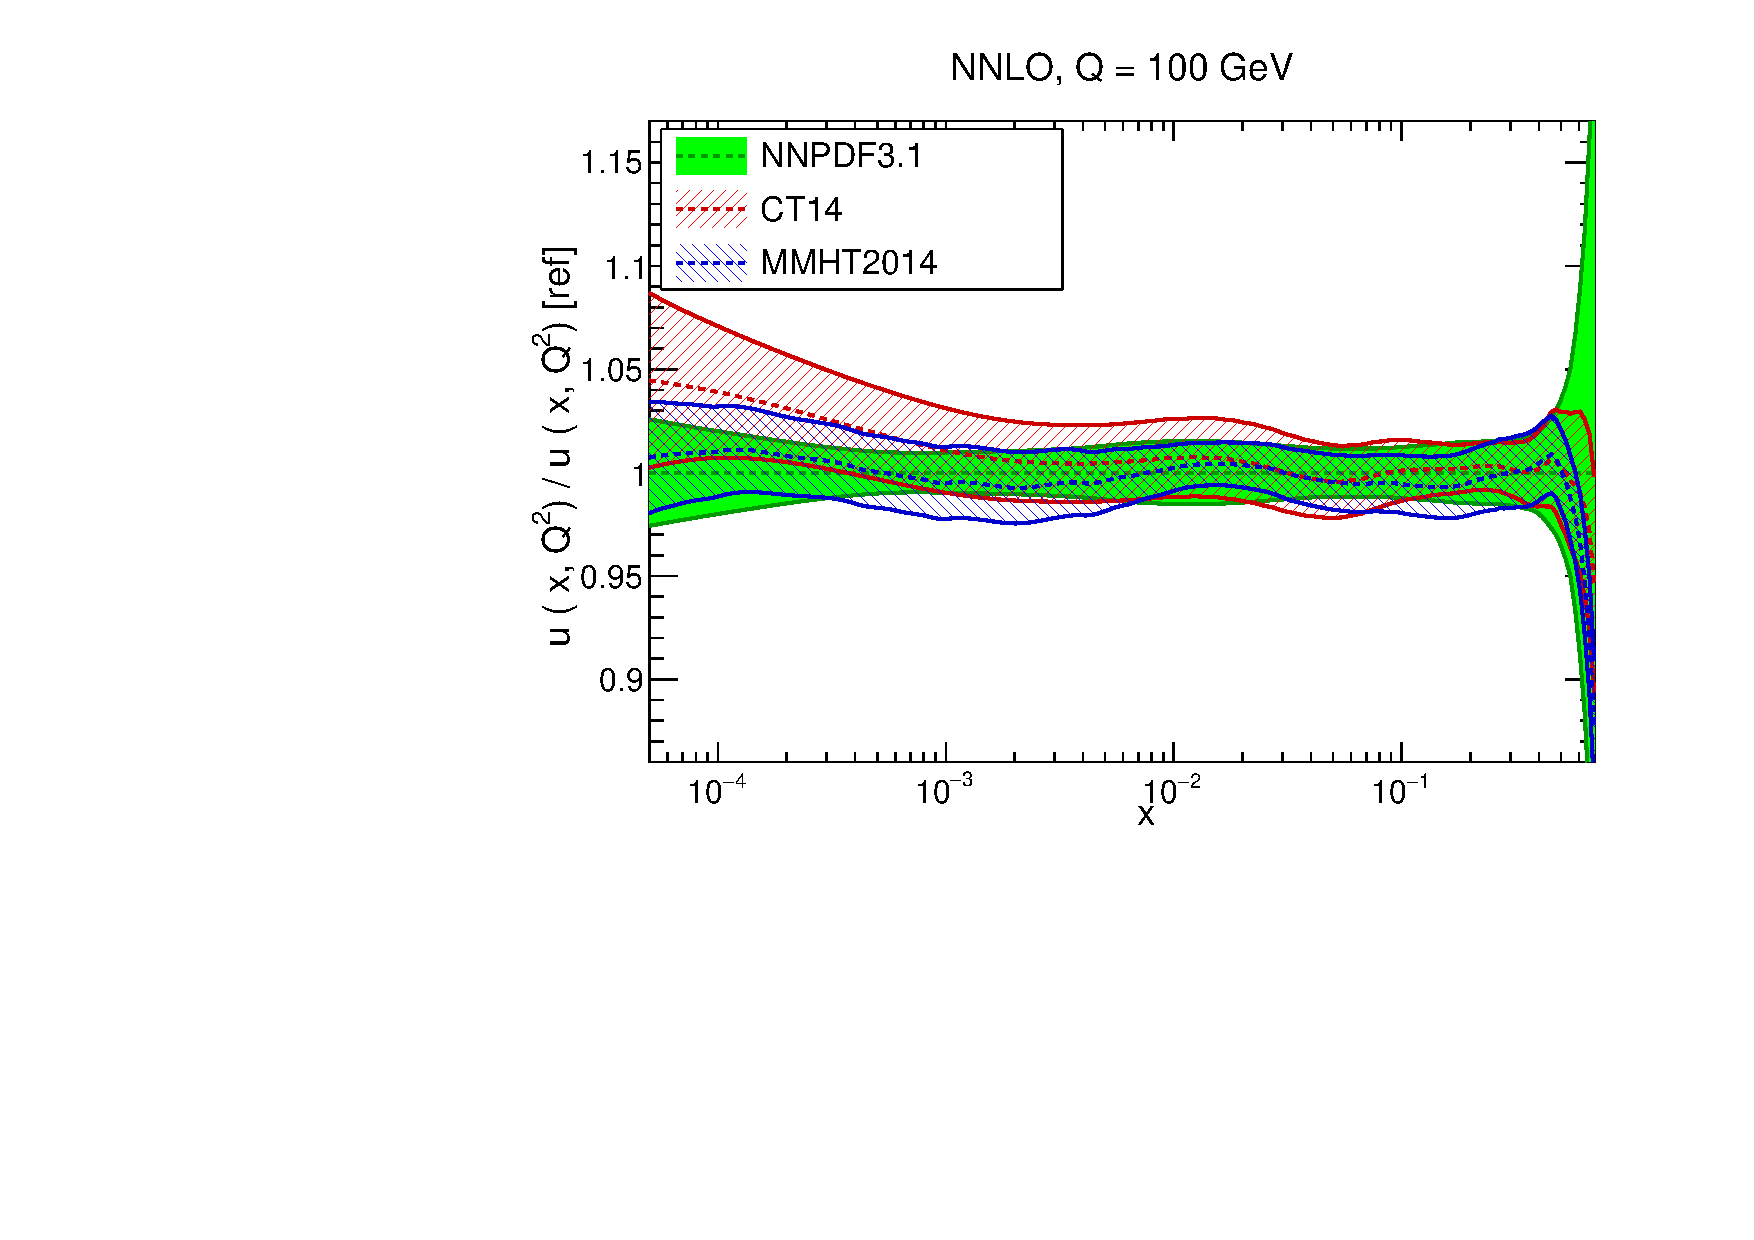
\includegraphics[scale=0.37]{plots/xu-31-nnlo-globalfits.pdf}
%    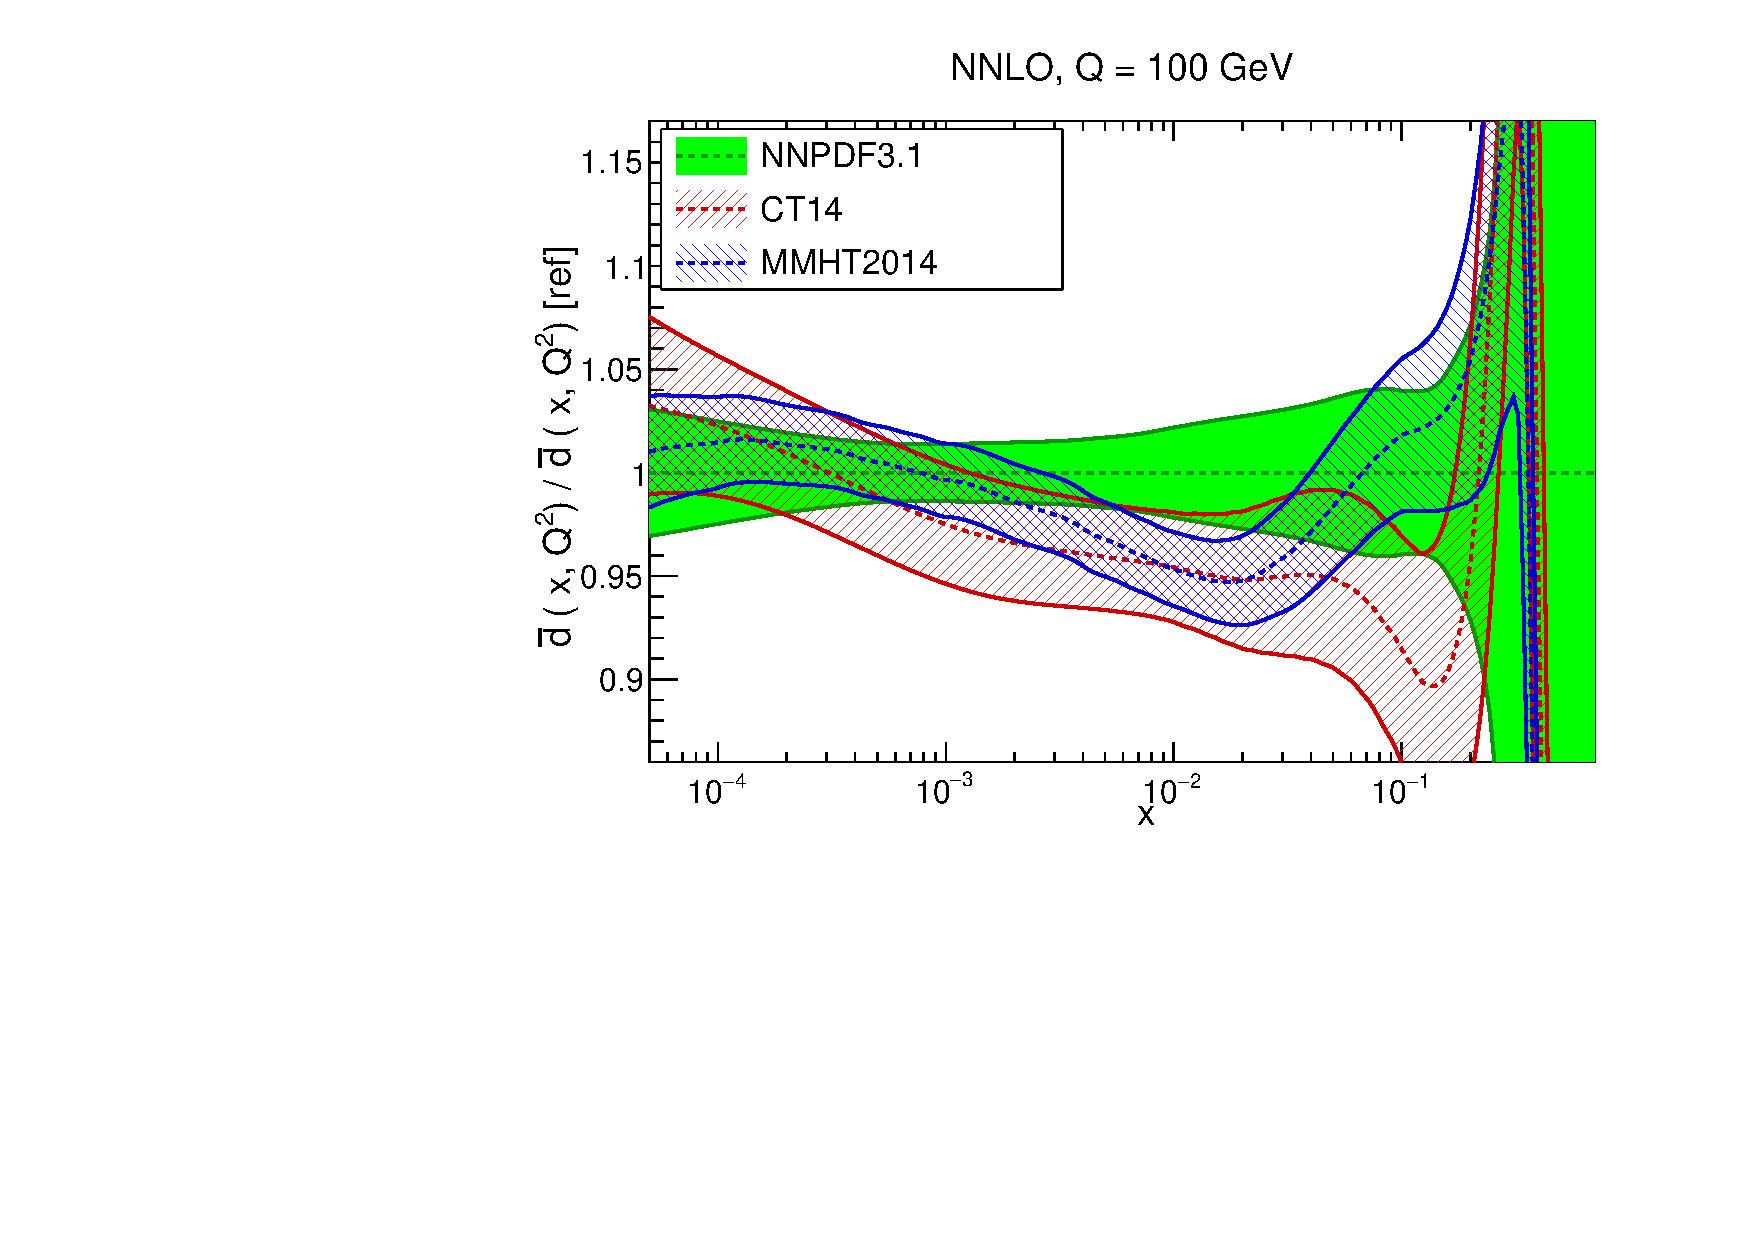
\includegraphics[scale=0.37]{plots/xdbar-31-nnlo-globalfits.pdf}
%  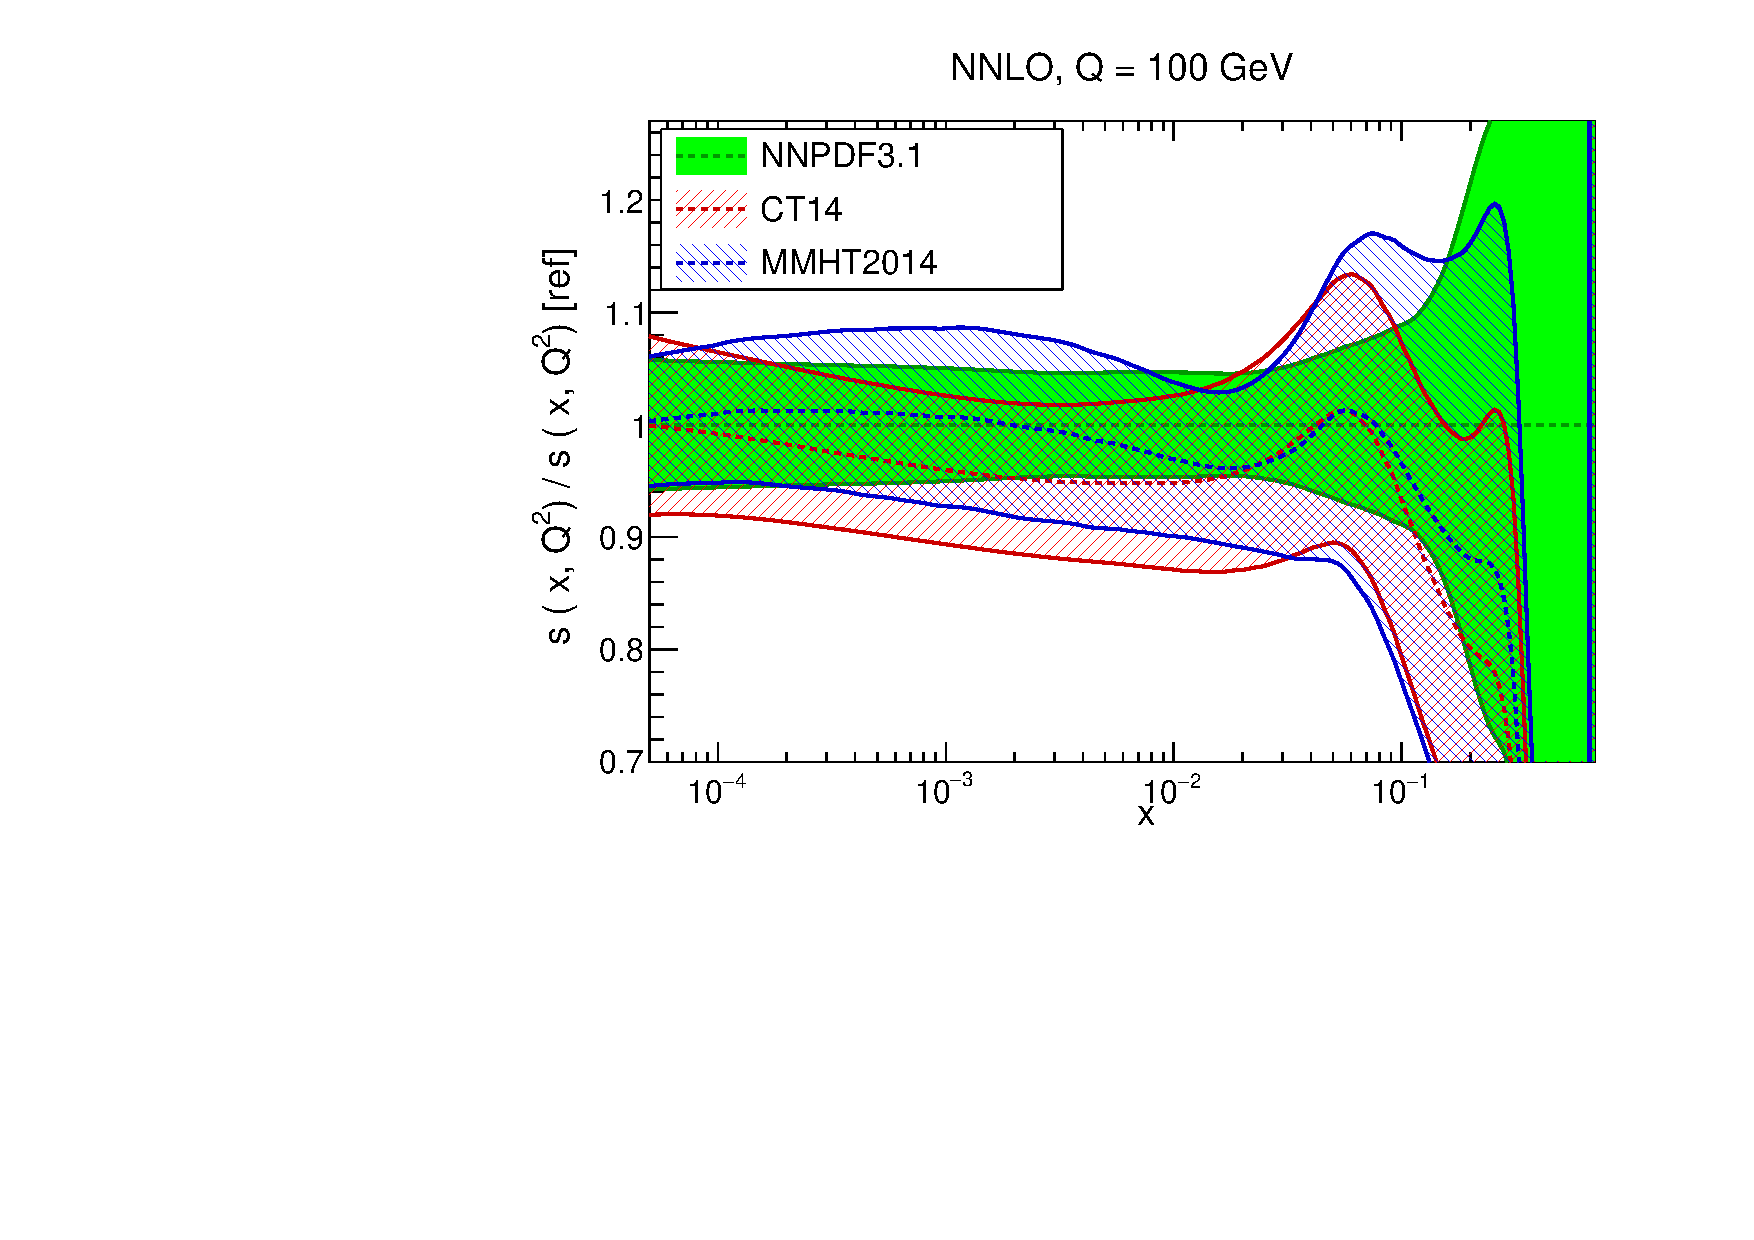
\includegraphics[scale=0.37]{plots/xs-31-nnlo-globalfits.pdf}
%   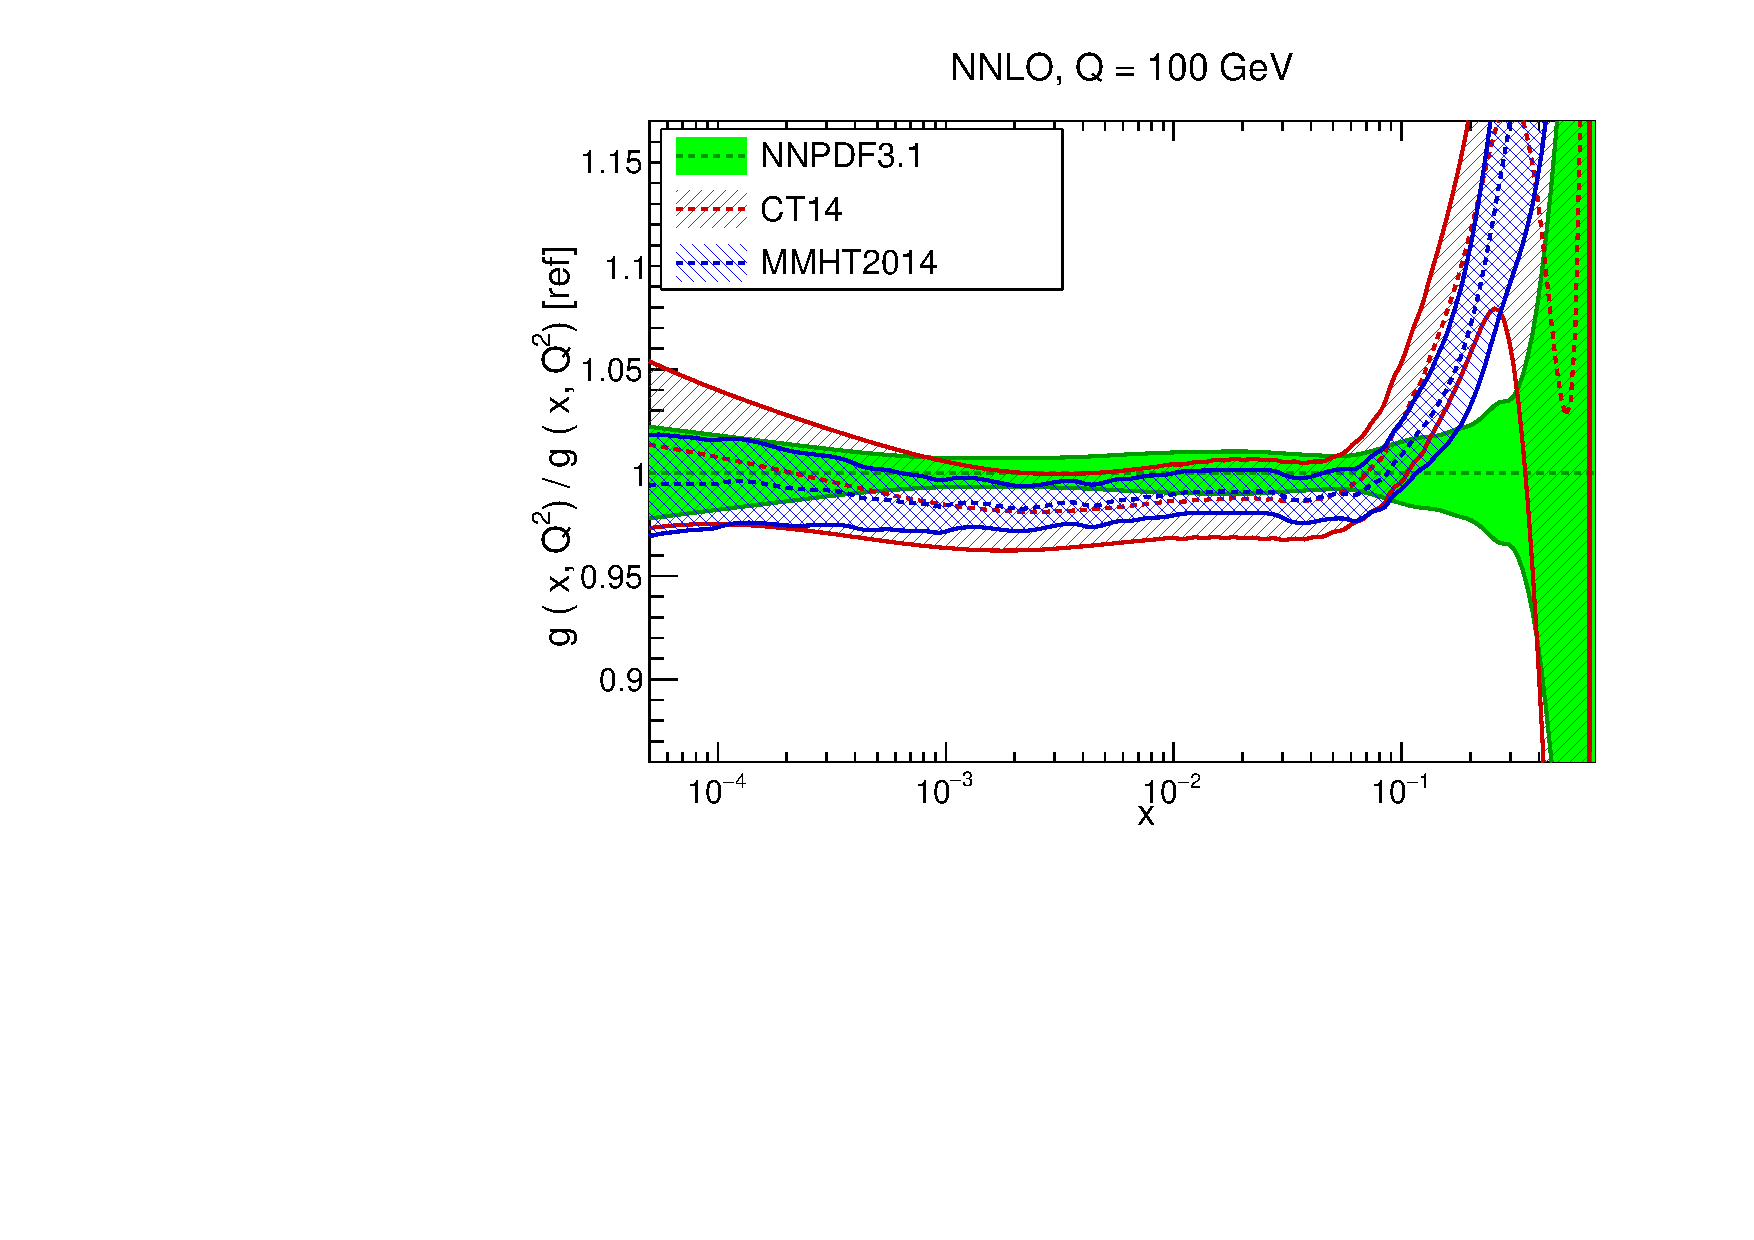
\includegraphics[scale=0.37]{plots/xg-31-nnlo-globalfits.pdf}
%  \caption{\small Comparison between the CT14, MMHT2014
%  and NNPDF3.1 NNLO PDF sets at $Q=100$ GeV, normalised
%  to the central value of the latter.
%  %
%  From top to bottom and from left to right we show the
%  $u$, $\bar{d}$ and $s$ quark PDFs as well as the gluon.
%  %
%  The error bands indicate the 1-$\sigma$ PDF uncertainties
%  associated to each set.
%  %
%  These PDF comparison plots have been produced using the
%  {\tt APFEL-Web} online plotting interface~\cite{Carrazza:2014gfa}.
%    \label{fig:globalfits}
%  }
%\end{center}
%\end{figure}
%%%%%%%%%%%%%%%%%%%%%%%%%%%%%%%%%%%%%%%%%%%%%%%%%%%%%%%%%%%%%%%%%%%%%%
%
%In addition to these latest versions of the global PDF fits,
%there has recently been a significant development of techniques aiming
%to construct combined PDF sets that are based on
%a small number of Hessian eigenvectors or MC replicas and thus
%are more efficient to use in lengthy higher-order
%computations or Monte Carlo simulations.
%%
%In particular, the PDF4LHC15 PDF sets are based on the
%combination of the CT14, MMHT14 and NNPDF3.1 NNLO PDF sets,
%subsequently reduced to a small number of eigenvectors
%(replicas) using the META-PDF~\cite{Gao:2013bia}
%and MC2H~\cite{Carrazza:2015aoa}
%(CMC~\cite{Carrazza:2015hva}) compression algorithms.
%%
%In this respect, Specialized Minimal PDF sets~\cite{Carrazza:2016htc}
%(SM-PDFs) have also
%been advocated, which
%are tailored to specific physical processes and are based
%on the minimal number of Hessian eigenvectors.
%%
%The PDF4LHC15 sets provide a suitable representative for the expectations
%from the global QCD analysis point of view, and as such will be used
%in the benchmark comparisons of the next section.
%
%Finally, and particularly relevant for the discussions in this white-paper,
%we strongly encourage the community to use the most recent versions
%of global PDF fits when comparing with existing or new
%lattice QCD calculations.
%%
%Comparing with deprecated sets, based on obsolete methodology
%and in many cases experimental data that has already been
%superseded, should always be avoided.
